% ============================================================
% T-DOME Paper I: The Seed
% T-DOME three-paper series, Paper I
% ============================================================

\documentclass[12pt]{article}
\usepackage[margin=1in]{geometry}
\usepackage{amsmath,amssymb,amsthm}
\usepackage[hidelinks]{hyperref}
\usepackage{booktabs}
\usepackage{physics}
\usepackage{graphicx}
\usepackage{caption}
\usepackage{array}
\newcolumntype{P}[1]{>{\raggedright\arraybackslash}p{#1}}
\graphicspath{{TDOME_I_supplement/}}

% Theorem environments — matching HAFF/Q-RAIF style
\newtheorem{theorem}{Theorem}
\newtheorem{lemma}[theorem]{Lemma}
\newtheorem{proposition}[theorem]{Proposition}
\newtheorem{definition}[theorem]{Definition}
\newtheorem{remark}[theorem]{Remark}
\newtheorem{corollary}[theorem]{Corollary}
\newtheorem{conjecture}[theorem]{Conjecture}

\title{Non-Markovian Memory and Temporal Accumulation:\\
A Conditional Thermodynamic Analysis}

\author{Sidong Liu, PhD \\
\small iBioStratix Ltd \\
\small \texttt{sidongliu@hotmail.com}}

\date{July 2026}

\begin{document}
\emergencystretch=2em
\raggedbottom
\hbadness=10000
\vbadness=10000
\maketitle

% ============================================================
\begin{abstract}
We investigate a conditional thermodynamic role for memory in open
quantum systems interacting with stochastic environments.  Working
within stochastic and information thermodynamics, we define a
\emph{survival functional} $\mathcal{S}:=\Delta F-W$ measuring the
difference between non-equilibrium free energy gained and work invested
by an agent.

For a fixed-Hamiltonian autonomous Davies/GKSL baseline with no
measurement or feedback, we prove a restricted Markovian ceiling:
$\mathcal{S}\leq0$.  This is not a universal ceiling for driven or
feedback-controlled Markovian agents.  We then derive an accounting
identity for finite-dimensional autonomous evolution, with the
interaction-energy term retained or a declared weak-coupling
approximation made, expressing the survival functional through changes
in system--environment mutual information and bath displacement.  In
models where prior interaction has supplied usable correlations, their
consumption during non-Markovian backflow intervals can yield
$\mathcal{S}>0$, bounded by the initial correlation budget.

The result is therefore a conditional memory advantage, not a proof that
memory or non-Markovianity is necessary or sufficient for all persistent
systems.  Fisher accretion and the comparison with the accessibility
ordering of the Holographic Alaya-Field Framework (HAFF) are presented
as heuristics.  A worked spin-boson example with Lorentz--Drude spectral
density illustrates how the accounting can operate in one supplied
model.

Finally, using entropy rate and predictive information from
computational mechanics, we study the implementation cost of a specified
irreversible archive-reset model.  Universal Landauer costs for merely
storing or maintaining memory, and the resulting universal ``Memory
Catastrophe,'' are withdrawn; only the declared archive implementation
is charged.

\medskip
\noindent\textbf{Keywords}: non-Markovian dynamics, open quantum systems,
Nakajima--Zwanzig equation, memory kernel, thermodynamic arrow of time,
information backflow, entropy production, stochastic thermodynamics
\end{abstract}

% ============================================================
\section{Introduction}
\label{sec:intro}

% ------------------------------------------------------------
\subsection{Context: The Problem of Persistence}

A quantum system coupled to a thermal environment generically
relaxes toward equilibrium. This is the content of the
\emph{zeroth crisis}: absent special structure, every open
subsystem is eventually erased by thermal noise~\cite{BreuerPetruccione2002}.

Yet the physical world contains persistent far-from-equilibrium
structures---from molecular machines to living organisms---that
maintain themselves against the entropic tide for timescales
vastly exceeding their intrinsic relaxation times. What
structural feature of their dynamics makes this possible?

The standard answer invokes free-energy input: a persistent system
continuously imports low-entropy energy and exports high-entropy
waste~\cite{Schrodinger1944}.  This paper asks the narrower accounting
question of when pre-existing system--environment correlations can fund
a later interval.  It does not claim that memory distinguishes every
persistent system from every non-persistent one.

% ------------------------------------------------------------
\subsection{Position within the Series}

This paper is the first of three constituting the
\textbf{T-DOME} (Thermodynamic Dynamics of Observer-Memory
Entanglement) framework, the third pillar of a three-paper
program.

\begin{center}
\small
\setlength{\tabcolsep}{4pt}%
\begin{tabular}{@{}lP{3.2cm}cP{3.4cm}c@{}}
\toprule
\textbf{Framework} & \textbf{Question} & & \textbf{Result} & \textbf{Status} \\
\midrule
HAFF~\cite{Liu2026HAFF_A,Liu2026HAFF_B}
  & How does geometry emerge?
  & Ocean
  & Conditional algebra/dictionary models
  & Revised \\[3pt]
Q-RAIF~\cite{Liu2026QRAIF_A,Liu2026QRAIF_B}
  & What algebra must an observer have?
  & Fish
  & Clifford representation as model input
  & Revised \\[3pt]
\textbf{T-DOME I} (this work)
  & What can inter-epoch correlations fund?
  & Seed
  & ELV-type accounting identity; restricted ceiling
  & \textbf{This paper} \\[3pt]
T-DOME II
  & How can a supplied archive be budgeted?
  & Ego
  & Conditional feature selection
  & Companion \\[3pt]
T-DOME III
  & When can residual statistics track drift?
  & Loop
  & Conditional Fisher calibration
  & Companion \\
\bottomrule
\end{tabular}
\end{center}

The three T-DOME papers form a conditional modelling sequence,
not an irreversible theorem chain:
\begin{enumerate}
\item \textbf{Paper I (The Seed):} The accounting identity asks when
  correlations built in earlier epochs can fund a later interval.
  A deliberately uncompressed archive is then introduced only as
  motivation for a finite-budget problem.
\item \textbf{Paper II (The Ego):} Given that archive model and a
  supplied component representation, Paper II studies conditional
  feature selection under a processing budget.
\item \textbf{Paper III (The Loop):} Given a selected frame and an
  explicit residual likelihood, Paper III studies conditions under
  which a calibration controller can track drift.
\end{enumerate}

\noindent
The present paper addresses only the first link in this chain.

% ------------------------------------------------------------
\subsection{Relation to HAFF Paper F}

Revised HAFF Paper F~\cite{Liu2026HAFF_F} treats record growth and
algebra inclusion as protocol-relative orderings and does not derive
a universal temporal partial order.  Section~\ref{sec:arrow} therefore
uses it only as motivation: a memory-influence relation and a
pointer-record ordering may be compared after both are supplied, but
neither is proved to embed in the other.

% ------------------------------------------------------------
\subsection{Scope and Disclaimers}

\begin{enumerate}
\item This work does \emph{not} claim that memory or
  non-Markovianity is necessary for persistence.  Continuously driven
  Markovian dissipative structures can persist.  The narrower claim is
  that pre-existing inter-epoch correlations can fund a positive
  interval of the survival accounting functional.
\item The sign of that functional is governed by changes in initial
  correlation and bath-displacement resources, not by Markovianity as
  such.  No strict comparison of Markovian and non-Markovian suprema is
  proved.
\item We do \emph{not} derive the specific form of the memory
  kernel from first principles. The kernel is treated as a
  structural feature of the system-environment coupling.
\item The term ``agent'' is used in the control-theoretic sense
  (a subsystem that acts on its environment to maintain a target
  state) and carries no implication of consciousness, intention,
  or subjective experience.
\item A broader structural analogy with classical philosophical
  concepts of temporal persistence exists but is outside the
  scope of this paper.
\end{enumerate}

\paragraph{Result-status ledger.}
The information--thermodynamic identity is a general finite-dimensional
unitary accounting identity (GvN/THM/OK-cond, with the interaction-energy
term retained or a declared weak-coupling approximation).  The original
time-dependent-control Markovian Ceiling is retracted; a narrower
autonomous Davies-semigroup theorem is proved below (FD/I/THM/OK-cond).
Fisher accretion and the HAFF bridge are heuristics.  Universal
Landauer costs for storing or maintaining memory and the resulting
``Memory Catastrophe'' are retracted; only a specified irreversible
archive-reset model remains.

% ============================================================
\section{Mathematical Preliminaries}
\label{sec:prelim}

% ------------------------------------------------------------
\subsection{Open Quantum Systems: The Markovian Baseline}

Consider a bipartite Hilbert space
$\mathcal{H} = \mathcal{H}_R \otimes \mathcal{H}_E$,
where $R$ denotes the ``agent'' (reduced system) and $E$ the
environment. The total Hamiltonian is
\begin{equation}
\label{eq:H_total}
H = H_R \otimes \mathbb{1}_E
  + \mathbb{1}_R \otimes H_E
  + \lambda\, H_{\mathrm{int}},
\end{equation}
where $\lambda$ parametrizes the coupling strength.

Under the Born--Markov and secular approximations, the reduced
dynamics of $\rho_R(t) = \mathrm{Tr}_E[\rho(t)]$ is governed by
the Gorini--Kossakowski--Sudarshan--Lindblad (GKSL) master
equation~\cite{Lindblad1976,GKS1976}:
\begin{equation}
\label{eq:GKSL}
\dot{\rho}_R(t)
= -i[H_{\mathrm{eff}},\, \rho_R(t)]
  + \sum_k \gamma_k \left(
    L_k \rho_R(t) L_k^\dagger
    - \tfrac{1}{2}\{L_k^\dagger L_k,\, \rho_R(t)\}
  \right),
\end{equation}
with $\gamma_k \geq 0$ and Lindblad operators $\{L_k\}$.

\begin{remark}[Markovian = Memoryless]
\label{rem:markov}
The GKSL equation is \emph{time-local}: $\dot{\rho}_R(t)$ depends
only on $\rho_R(t)$, never on $\rho_R(s)$ for $s < t$.
Physically, this corresponds to an environment with vanishing
correlation time ($\tau_E \to 0$): the bath ``forgets'' its
interaction with the system instantaneously.
The semigroup property $\Lambda(t+s) = \Lambda(t)\Lambda(s)$
ensures complete positivity at all times but precludes any
information backflow from environment to system~\cite{RivasHuelgaPlenio2014}.
\end{remark}

% ------------------------------------------------------------
\subsection{Beyond Markov: The Nakajima--Zwanzig Equation}

When the environmental correlation time $\tau_E$ is non-negligible,
the Born--Markov approximation fails. The exact reduced dynamics
is captured by the Nakajima--Zwanzig (NZ) integro-differential
equation~\cite{Nakajima1958,Zwanzig1960}:
\begin{equation}
\label{eq:NZ}
\dot{\rho}_R(t)
= -i[H_{\mathrm{eff}},\, \rho_R(t)]
  + \int_0^t ds\; \mathcal{K}(t,s)\, \rho_R(s),
\end{equation}
where $\mathcal{K}(t,s)$ is the \textbf{memory kernel}---a
superoperator encoding the influence of the system's entire
history on its present dynamics.

\begin{definition}[Memory Kernel]
\label{def:kernel}
The memory kernel $\mathcal{K}: [0,\infty)^2 \to
\mathcal{L}(\mathcal{B}(\mathcal{H}_R))$ is the superoperator
satisfying~\eqref{eq:NZ}. It encodes two types of information:
\begin{enumerate}
\item \textbf{Environmental structure:} the spectral density,
  correlation functions, and non-equilibrium features of the bath;
\item \textbf{Temporal reach:} the effective support
  $\tau_{\mathrm{mem}} := \inf\{\tau : \|\mathcal{K}(t,s)\| < \epsilon
  \;\forall\; t - s > \tau\}$, the ``memory depth.''
\end{enumerate}
The Markovian limit corresponds to
$\mathcal{K}(t,s) \to \mathcal{K}_0\, \delta(t-s)$,
recovering the GKSL generator.
\end{definition}

\begin{remark}[Information Backflow]
\label{rem:backflow}
Non-Markovian dynamics admits \emph{information backflow}:
the distinguishability of two initial states, as measured by
trace distance $D(\rho_1(t), \rho_2(t))$, can temporarily
increase~\cite{BreuerLainePiilo2009}. This is the operational
signature of memory---the environment returns previously
absorbed information to the system.
\end{remark}

% ------------------------------------------------------------
\subsection{Thermodynamic Framework}
\label{subsec:thermo}

We adopt the framework of stochastic thermodynamics for open
quantum systems~\cite{EspositoLindenbergVandenBroeck2010}.
The following conventions are fixed throughout.

\begin{definition}[Thermodynamic Setup]
\label{def:thermo_setup}
\leavevmode
\begin{enumerate}
\item \textbf{Hamiltonian decomposition.}
  The system Hamiltonian is
  $H_S(t) = H_R + H_{\mathrm{ctrl}}(t)$,
  where $H_R$ is the \emph{fixed} bare Hamiltonian and
  $H_{\mathrm{ctrl}}(t)$ is the agent's time-dependent
  control protocol.
  The bath Hamiltonian $H_E$ and coupling $H_{\mathrm{int}}$
  are as in~\eqref{eq:H_total}.

\item \textbf{Reference state.}
  The thermal equilibrium state of the bare Hamiltonian is
  \begin{equation}
  \label{eq:rho_eq}
  \rho_{\mathrm{eq}} := \frac{e^{-\beta H_R}}{Z_R},
  \qquad Z_R := \tr(e^{-\beta H_R}),
  \qquad \beta := (k_B T)^{-1}.
  \end{equation}
  Since $H_R$ is time-independent, $\rho_{\mathrm{eq}}$ is a
  well-defined, fixed reference throughout the protocol.

\item \textbf{Non-equilibrium free energy.}
  For any state $\rho$ of the reduced system,
  \begin{equation}
  \label{eq:F_neq}
  F(\rho) := \tr(\rho\, H_R) + \beta^{-1}\tr(\rho\ln\rho)
  = \langle H_R \rangle_\rho - \beta^{-1} S(\rho),
  \end{equation}
  where $S(\rho) = -\tr(\rho\ln\rho)$ is the von~Neumann entropy.
  The equilibrium value is $F_{\mathrm{eq}} = -\beta^{-1}\ln Z_R$.

\item \textbf{Free energy--relative entropy identity.}
  \begin{equation}
  \label{eq:DKL_F}
  D_{\mathrm{KL}}(\rho \| \rho_{\mathrm{eq}})
  = \beta\bigl(F(\rho) - F_{\mathrm{eq}}\bigr) \geq 0.
  \end{equation}
  Thus $D_{\mathrm{KL}}$ measures the free-energy surplus in
  units of $k_B T$.

\item \textbf{Work.}
  The inclusive work performed on the total system by the control protocol
  over $[0,\tau]$ is
  \begin{equation}
  \label{eq:work}
  W[0,\tau] := \int_0^\tau
  \tr\!\left(\rho(t)\,
  \frac{\partial H_{\mathrm{ctrl}}}{\partial t}\right) dt.
  \end{equation}

\item \textbf{Entropy-production functional.}
  The \emph{generalised entropy production} over $[0,\tau]$ is
  \begin{equation}
  \label{eq:Sigma}
  \Sigma[0,\tau] := \beta\bigl(W[0,\tau] - \Delta F\bigr),
  \end{equation}
  where $\Delta F = F(\rho(\tau)) - F(\rho(0))$.
  For uncorrelated (product) initial states,
  $\Sigma \geq 0$ recovers the standard second-law bound.
  For initially correlated states, $\Sigma$ can be
  \emph{negative}, reflecting the consumption of
  pre-existing correlations
  (see Remark~\ref{rem:battery}).
\end{enumerate}
\end{definition}

\begin{remark}[Why $H_R$ is fixed]
\label{rem:H_fixed}
The bare Hamiltonian $H_R$ defines the system's energy scale and
hence the reference state $\rho_{\mathrm{eq}}$.
The agent acts on the world through $H_{\mathrm{ctrl}}(t)$,
which may be time-dependent.
This separation ensures that $\rho_{\mathrm{eq}}$ is
well-defined and time-independent for the accounting identity.
It does \emph{not} make a driven generator satisfy detailed balance
with respect to that fixed state.  The ceiling result below therefore
uses autonomous $H_{\mathrm{ctrl}}=0$ dynamics.
\end{remark}

\begin{definition}[Standing Assumptions]
\label{def:assumptions}
The following minimal assumptions are in force throughout
Sections~\ref{sec:advantage}--\ref{sec:example} unless
stated otherwise.
Every main result
(Lemma~\ref{lem:info_thermo},
Theorem~\ref{thm:advantage},
Corollary~\ref{cor:three_regimes})
relies \emph{only} on items
\textup{(A1)--(A5)} below.
\begin{enumerate}
\item[\textup{(A1)}]
  \textbf{Finite-dimensional bipartite system.}
  $\mathcal{H} = \mathcal{H}_S \otimes \mathcal{H}_E$,
  with total Hamiltonian~\eqref{eq:H_total}
  and global unitary evolution
  $U(t) = \mathcal{T}\exp(-i\int_0^t H(s)\,ds)$.

\item[\textup{(A2)}]
  \textbf{Weak coupling.}
  The system--environment interaction satisfies
  $\lambda \ll 1$ in~\eqref{eq:H_total}, so that
  $\Delta\langle H_{\mathrm{int}} \rangle
  = O(\lambda)$~\cite{BreuerPetruccione2002}.
  The first-law bookkeeping is
  $W=\Delta\langle H_R\rangle
  + \Delta\langle H_{\mathrm{ctrl}}\rangle
  + \Delta\langle H_E\rangle
  + \Delta\langle H_{\mathrm{int}}\rangle$.
  Dropping the last term is the declared weak-coupling approximation
  $\Delta\langle H_{\mathrm{int}}\rangle=O(\lambda)$; it is not
  an energy-conservation equation with a zero right-hand side.

\item[\textup{(A3)}]
  \textbf{Fixed environmental reference.}
  $\rho_E^{\mathrm{th}} := e^{-\beta H_E}/Z_E$
  is a fixed \emph{bookkeeping} Gibbs state at inverse
  temperature $\beta$.
  The \emph{actual} initial bath state $\rho_E(0)$
  need not coincide with $\rho_E^{\mathrm{th}}$;
  when $\rho_E(0) \neq \rho_E^{\mathrm{th}}$, the quantity
  $D_{\mathrm{KL}}(\rho_E(t)\|\rho_E^{\mathrm{th}})$
  tracks the nonequilibrium free energy stored in the bath
  relative to this reference.
  The bath Hamiltonian $H_E$ is time-independent.

\item[\textup{(A4)}]
  \textbf{Arbitrary initial state.}
  The total initial state $\rho_{SE}(0)$ is \emph{not}
  required to be a product state.
  In particular, initial system--environment correlations
  $I(S{:}E;\,0) > 0$ and initial bath displacement
  $D_{\mathrm{KL}}(\rho_E(0)\|\rho_E^{\mathrm{th}}) > 0$
  are both permitted.
\item[\textup{(A5)}]
  \textbf{Regularity.}
  All quantum states appearing in the thermodynamic
  identities are assumed to have full rank (or are
  restricted to their support), so that all relative
  entropies $D_{\mathrm{KL}}(\rho\|\sigma)$ are finite.
\end{enumerate}
\end{definition}

\begin{remark}[Bookkeeping conventions]
\label{rem:bookkeeping}
The heat absorbed by the environment is
$Q := \Delta\langle H_E \rangle
= \mathrm{Tr}[\rho_E(\tau) H_E]
  - \mathrm{Tr}[\rho_E(0) H_E]$
(matching
Esposito \emph{et al.}~\cite{EspositoLindenbergVandenBroeck2010}).
We define $\Sigma := \beta(W - \Delta F)$ as a
\emph{generalised entropy-balance functional};
for correlated initial conditions $\Sigma$ need not be
nonnegative
(see Remark~\ref{rem:battery}).
\end{remark}

% ------------------------------------------------------------
\subsection{The Survival Functional}
\label{subsec:survival}

We now define the central quantity of this paper.

\begin{definition}[Survival Functional]
\label{def:survival}
For a reduced system $R$ evolving under dynamics $\Lambda$
over $[0,\tau]$, the \textbf{survival functional} is
\begin{equation}
\label{eq:survival}
\mathcal{S}[\Lambda, \tau]
:= \Delta F - W[0,\tau]
= \bigl[F(\rho(\tau)) - F(\rho(0))\bigr] - W[0,\tau].
\end{equation}
Equivalently, using~\eqref{eq:Sigma},
\begin{equation}
\label{eq:survival_Sigma}
\beta\,\mathcal{S}[\Lambda,\tau] = -\Sigma[0,\tau].
\end{equation}
\end{definition}

\noindent\textit{Note on nomenclature.}
We retain the term ``survival functional'' to emphasize
the biological interpretation of persistence far from
equilibrium; mathematically, $\mathcal{S}$ is strictly a
\emph{generalized entropy-balance functional} derived from
the first and second laws.

\begin{remark}[Interpretation]
\label{rem:survival_interp}
The survival functional has a transparent physical meaning:
\begin{itemize}
\item $\mathcal{S} > 0$: the system gained more free energy than
  was invested by the external protocol---a \emph{thermodynamic
  profit}. The agent has extracted usable work from environmental
  correlations.
\item $\mathcal{S} = 0$: the agent breaks even (reversible limit,
  $\Sigma = 0$).
\item $\mathcal{S} < 0$: the agent paid more than it gained
  (the generic irreversible case).
\end{itemize}
Under the standard second law ($\Sigma \geq 0$),
$\mathcal{S} \leq 0$ always.
As Section~\ref{sec:advantage} shows, a positive interval requires
consumption of a resource present at that interval's initial time,
such as system--environment correlation or bath displacement.
Whether a memory kernel preserves access to that resource is a
model-specific dynamical question.
\end{remark}

\begin{remark}[Connection to Information Thermodynamics]
\label{rem:connection_SU}
In the Sagawa--Ueda framework~\cite{SagawaUeda2010,SagawaUeda2012},
a system under feedback control satisfies the generalized second law
\begin{equation}
\label{eq:sagawa_ueda}
\Sigma \geq -I_{\mathrm{feedback}},
\end{equation}
where $I_{\mathrm{feedback}} \geq 0$ is the mutual information
gained through measurement of the system.
This permits $\Sigma < 0$ (and hence $\mathcal{S} > 0$) at
the expense of information.
Pre-existing correlations can enter the entropy balance in a role
analogous to measurement information.  A memory kernel is not
automatically a measurement or feedback controller; a concrete model
must show that it preserves and later exposes those correlations.
\end{remark}

% ============================================================
\section{A Restricted Markovian Baseline}
\label{sec:ceiling}

The former ``Markovian Ceiling'' allowed a time-dependent control
Hamiltonian while using a fixed bare Gibbs state as the
detailed-balance reference.  A driven generator need not preserve that
state, so the asserted balance law did not follow from Spohn's
inequality.  That theorem, its open-loop control class, and its
temporal-blindness corollary are retracted.  The autonomous result below
is the narrower statement that survives.

\subsection{Spohn's Inequality}

Throughout this section we assume that the GKSL generator
$\mathcal{L}$ is a \emph{thermal Lindbladian}: it is obtained
from the weak-coupling (Davies) limit of a system coupled to a
single thermal bath at inverse temperature $\beta$, and satisfies
\textbf{quantum detailed balance} (the KMS
condition)~\cite{Spohn1978,BreuerPetruccione2002}.
Under this assumption, the unique stationary state is the Gibbs
state $\rho_{\mathrm{ss}} = \rho_{\mathrm{eq}}$
of~\eqref{eq:rho_eq}, and the generator is self-adjoint with
respect to the KMS inner product.
This ensures that the entropy production rate below is
well-defined and non-negative.

\begin{definition}[Autonomous Davies baseline]
\label{def:autonomous_davies}
The autonomous baseline has $H_{\mathrm{ctrl}}=0$, fixed system
Hamiltonian $H_R$, and a time-independent Davies/GKSL generator
$\mathcal L$ satisfying quantum detailed balance with respect to the
faithful Gibbs state $\rho_{\mathrm{eq}}=e^{-\beta H_R}/Z_R$.
No measurement, feedback, or initial system--bath resource is included
in this reduced semigroup model.
\end{definition}

\begin{lemma}[Spohn~\cite{Spohn1978}]
\label{lem:spohn}
For any GKSL dynamical semigroup $\Lambda_t = e^{\mathcal{L}t}$
satisfying quantum detailed balance with unique invariant state
$\rho_{\mathrm{eq}}$, the entropy production
rate
\begin{equation}
\label{eq:spohn_sigma}
\sigma(t) := -\tr\!\bigl(\mathcal{L}[\rho(t)]\,
(\ln\rho(t) - \ln\rho_{\mathrm{eq}})\bigr)
\end{equation}
satisfies $\sigma(t) \geq 0$, equivalently
$dD_{\mathrm{KL}}(\rho(t)\|\rho_{\mathrm{eq}})/dt\leq0$.
\end{lemma}

\begin{proof}
This follows from the contractivity of CPTP maps under quantum
relative entropy~\cite{Spohn1978,BreuerPetruccione2002}:
$D_{\mathrm{KL}}(\Lambda_t\rho \| \Lambda_t\rho_{\mathrm{eq}})
\leq D_{\mathrm{KL}}(\rho \| \rho_{\mathrm{eq}})$
for all $t \geq 0$.
Differentiating at $t = 0$ yields $\sigma(t) \geq 0$.
\end{proof}

\subsection{The Restricted Autonomous Ceiling}

\begin{theorem}[Restricted Autonomous Ceiling]
\label{thm:autonomous_ceiling}
Under Definition~\ref{def:autonomous_davies}, the survival functional
obeys
\begin{equation}
\label{eq:ceiling}
\mathcal S[0,\tau]=F(\rho(\tau))-F(\rho(0))\leq0.
\end{equation}
Equality requires no decrease of relative entropy on the interval
(for a primitive semigroup, equilibrium is the stationary equality case).
\end{theorem}

\begin{proof}
Here $W=0$.  By~\eqref{eq:DKL_F} and Lemma~\ref{lem:spohn},
$\beta\Delta F=\Delta D_{\mathrm{KL}}\leq0$, hence
$\mathcal S=\Delta F\leq0$.
\end{proof}

\begin{remark}[Driven protocols require a different theorem]
\label{rem:driven_protocol}
For time-dependent $H_S(t)$ one may define the instantaneous Gibbs
state of the full driven Hamiltonian and assume a generator satisfying
instantaneous detailed balance, together with inclusive work
$\int\tr(\rho\,\dot H_S)dt$.  Those hypotheses describe a different
driven-thermodynamics result and are not proved here.  Open-loop alone
does not repair the missing relation between generator and reference
state; feedback protocols require their own information balance.
\end{remark}

\begin{remark}[Memorylessness and temporal correlations]
\label{rem:temporal_blindness}
Under the Born--Markov approximation, the bath correlation
function is replaced by its white-noise limit
$C(t,s) \to C_0\,\delta(t-s)$, and the GKSL dissipator depends
only on the spectral density $J(\omega)$ evaluated at the
system's Bohr frequencies.
The reduced semigroup therefore omits explicit inter-epoch bath
correlations.  This modelling loss does not imply a universal spectral
gap formula, a universal maintenance-work bound, or impossibility of
continuously driven Markovian persistence.
\end{remark}

\begin{remark}[Dissipative vs.\ Self-Nourishing Structures]
\label{rem:ceiling_physics}
The restricted theorem is a free-energy monotonicity statement for one
autonomous detailed-balance class.  It does not say that Markovian
systems cannot persist under continuous driving, that non-Markovianity
is necessary for persistence, or that a memory kernel alone supplies
usable feedback.  It is a controlled baseline for comparisons at fixed
initial resources.
\end{remark}

% ============================================================
\section{Initial-Correlation Accounting}
\label{sec:advantage}

We now separate a dynamics-agnostic accounting identity from the
model-dependent question of memory.  Quantum mutual information
$I(S{:}E)$ can be a consumable initial resource.  A non-Markovian model
may preserve such a resource across epochs, but non-Markovianity alone
does not fix the sign of $\mathcal S$ and is neither necessary nor
sufficient for a positive interval.

\subsection{System--Environment Mutual Information}

We work with the total system--environment state
$\rho_{SE}(t)$, evolving unitarily under the total
Hamiltonian~\eqref{eq:H_total}.
The quantum mutual information
\begin{equation}
\label{eq:mutual_info}
I(S{:}E;\, t) := S(\rho_S(t)) + S(\rho_E(t))
  - S(\rho_{SE}(t))
= D_{\mathrm{KL}}\!\bigl(\rho_{SE}(t) \,\big\|\,
  \rho_S(t) \otimes \rho_E(t)\bigr)
\geq 0
\end{equation}
quantifies the total correlations (classical and quantum)
between the system $S$ and the environment $E$ at time $t$.

\begin{remark}[Role of Initial Correlations]
\label{rem:initial_corr}
Under the Born approximation, the initial state is taken as a
product $\rho_{SE}(0) = \rho_S(0) \otimes \rho_E^{\mathrm{th}}$,
so $I(S{:}E;\, 0) = 0$.
For a system already interacting with its environment, a restart state
\emph{may} be correlated.  If a specified memory mechanism preserves
those correlations and a later interval consumes them, they contribute
to that interval's resource balance.  This is a conditional mechanism,
not a generic property of every persistent system or memory kernel.
\end{remark}

\subsection{The Information--Thermodynamic Identity}

The following identity is the central technical tool of this
section.
It holds for \textbf{any} initial state---product or
correlated---and relies only on unitarity and the definitions
of mutual information and relative entropy.
It is the Esposito--Lindenberg--Van den Broeck entropy-production
decomposition~\cite{EspositoLindenbergVandenBroeck2010}, written so
that arbitrary initial-correlation terms are retained explicitly.

\begin{remark}[Relative-entropy chain rule]
\label{rem:chain_rule}
We repeatedly use the identity
\begin{equation}
\label{eq:chain_general}
D_{\mathrm{KL}}\!\bigl(\rho_{SE}\,\big\|\,
  \rho_S\otimes\sigma_E\bigr)
= I(S{:}E)_{\rho_{SE}}
  + D_{\mathrm{KL}}(\rho_E\|\sigma_E),
\end{equation}
valid for \emph{arbitrary} (possibly correlated)
$\rho_{SE}$ and any full-rank reference state
$\sigma_E$.\footnote{This follows from the definition of
quantum relative entropy and
$\ln(\rho_S\otimes\sigma_E)
= \ln\rho_S\otimes\mathbb{1}_E
  +\mathbb{1}_S\otimes\ln\sigma_E$.
See, e.g., M.~M.~Wilde, \emph{Quantum Information
Theory}, 2nd ed., Cambridge University Press (2017),
Sec.~11; and M.~A.~Nielsen and I.~L.~Chuang,
\emph{Quantum Computation and Quantum Information},
Cambridge University Press (2000), Ch.~11.}
Importantly, this is a \emph{pure algebraic identity} and
does not assume product initial conditions.
\end{remark}

\begin{lemma}[Information--Thermodynamic Identity]
\label{lem:info_thermo}
Let $\rho_{SE}(t)$ evolve unitarily under the total
Hamiltonian.
Then, for \textbf{any} initial state $\rho_{SE}(0)$
(product or correlated):
\begin{equation}
\label{eq:info_thermo}
\Delta I(S{:}E)
+ \Delta D_{\mathrm{KL}}\!\bigl(\rho_E \,\big\|\,
  \rho_E^{\mathrm{th}}\bigr)
= \Delta S_S + \beta\,\Delta\langle H_E \rangle,
\end{equation}
where $\Delta S_S = S(\rho_S(\tau)) - S(\rho_S(0))$ is the
change in the system's von~Neumann entropy and
$\Delta\langle H_E \rangle
= \mathrm{Tr}[\rho_E(\tau)\, H_E]
  - \mathrm{Tr}[\rho_E(0)\, H_E]$
is the energy absorbed by the environment.
\end{lemma}

\begin{proof}
Applying the chain rule~\eqref{eq:chain_general}
(Remark~\ref{rem:chain_rule}) with
$\sigma_E = \rho_E^{\mathrm{th}}$:
\begin{equation}
\label{eq:chain_step}
D_{\mathrm{KL}}\!\bigl(\rho_{SE}(t) \,\big\|\,
  \rho_S(t) \otimes \rho_E^{\mathrm{th}}\bigr)
= I(S{:}E;\, t)
  + D_{\mathrm{KL}}\!\bigl(\rho_E(t) \,\big\|\,
    \rho_E^{\mathrm{th}}\bigr).
\end{equation}
Expanding the left side using
$\ln\rho_E^{\mathrm{th}} = -\beta H_E - \ln Z_E$:
\begin{equation}
\label{eq:phi_expand}
D_{\mathrm{KL}}\!\bigl(\rho_{SE}(t) \,\big\|\,
  \rho_S(t) \otimes \rho_E^{\mathrm{th}}\bigr)
= -S(\rho_{SE}(t)) + S(\rho_S(t))
  + \beta\langle H_E \rangle_t + \ln Z_E.
\end{equation}
Since the total evolution is unitary,
$S(\rho_{SE}(t)) = S(\rho_{SE}(0))$ for all $t$.
Taking the difference between times $\tau$ and $0$ cancels
both $S(\rho_{SE})$ and $\ln Z_E$, yielding
\begin{equation}
\Delta\!\left[I(S{:}E)
  + D_{\mathrm{KL}}(\rho_E \| \rho_E^{\mathrm{th}})\right]
= \Delta S_S + \beta\,\Delta\langle H_E \rangle.
\end{equation}
\end{proof}

\begin{remark}[No assumption on the initial state]
\label{rem:no_product_lemma}
The proof of Lemma~\ref{lem:info_thermo} uses \emph{only}
unitarity ($\Delta S(\rho_{SE}) = 0$) and the algebraic
structure of the KL divergence.
No assumption is made about the initial state $\rho_{SE}(0)$,
the coupling strength, or the character (Markovian or
non-Markovian) of the reduced dynamics.
For a product thermal initial state, autonomous driving, and negligible
endpoint interaction energy, the associated entropy balance reduces to
the Esposito decomposition~\cite{EspositoLindenbergVandenBroeck2010}:
$\Sigma = I(S{:}E;\,\tau)
+ D_{\mathrm{KL}}(\rho_E(\tau) \| \rho_E^{\mathrm{th}})
+O(\lambda)$.
\end{remark}

\subsection{The Survival Identity}

We now connect the information--thermodynamic
identity~\eqref{eq:info_thermo} to the survival
functional $\mathcal{S}$ defined in
Section~\ref{subsec:survival}.

\begin{theorem}[Survival Balance: General Form]
\label{thm:advantage}
Under Assumptions \textup{(A1)--(A5)} of
Definition~\ref{def:assumptions},
let $\rho_{SE}(t)$ evolve unitarily from an \emph{arbitrary}
(possibly correlated) initial state $\rho_{SE}(0)$.
The survival functional
satisfies
\begin{equation}
\label{eq:advantage}
\boxed{\;
\beta\,\mathcal{S}[\Lambda,\tau]
= -\Delta I(S{:}E)
  - \Delta D_{\mathrm{KL}}\!\bigl(\rho_E \,\big\|\,
    \rho_E^{\mathrm{th}}\bigr)
  - \beta\,\Delta\langle H_{\mathrm{ctrl}} \rangle
  - \beta\,\Delta\langle H_{\mathrm{int}} \rangle,
\;}
\end{equation}
where $\Delta\langle H_{\mathrm{ctrl}} \rangle
= \mathrm{Tr}[\rho_S(\tau)\, H_{\mathrm{ctrl}}(\tau)]
  - \mathrm{Tr}[\rho_S(0)\, H_{\mathrm{ctrl}}(0)]$
is the change in the control-field energy.

For \textbf{autonomous evolution} with negligible interaction-energy
change at the endpoints
($H_{\mathrm{ctrl}} = 0$ and
$\Delta\langle H_{\mathrm{int}}\rangle=O(\lambda)$),
the weak-coupling form is
\begin{equation}
\label{eq:advantage_auto}
\beta\,\mathcal{S}[\Lambda,\tau]
= -\Delta I(S{:}E)
  - \Delta D_{\mathrm{KL}}\!\bigl(\rho_E \,\big\|\,
    \rho_E^{\mathrm{th}}\bigr)+O(\lambda).
\end{equation}
\end{theorem}

\begin{proof}
The proof uses three ingredients: the definition of
$\mathcal{S}$, the first law, and
Lemma~\ref{lem:info_thermo}.

\noindent\textbf{Step 1 (First law in weak coupling).}
Since $H_{\mathrm{ctrl}}(t)$ is the only explicitly time-dependent
component of $H$, inclusive work satisfies the exact first law
$W = \Delta\langle H \rangle
= \Delta\langle H_R \rangle
  + \Delta\langle H_{\mathrm{ctrl}} \rangle
  + \Delta\langle H_E \rangle
  + \Delta\langle H_{\mathrm{int}} \rangle$.

\noindent\textbf{Step 2 (Connecting $\Sigma$ to the
identity).}
From Definition~\ref{def:survival} and~\eqref{eq:Sigma},
using $\Delta F = \Delta\langle H_R \rangle
- \beta^{-1}\Delta S_S$:
\begin{align}
\Sigma &= \beta(W - \Delta F)
= \beta\bigl(W - \Delta\langle H_R \rangle\bigr)
  + \Delta S_S \nonumber \\
&= \beta\bigl(\Delta\langle H_{\mathrm{ctrl}} \rangle
  + \Delta\langle H_E \rangle
  + \Delta\langle H_{\mathrm{int}} \rangle\bigr) + \Delta S_S
\nonumber \\
&= \bigl(\Delta S_S
  + \beta\,\Delta\langle H_E \rangle\bigr)
  + \beta\,\Delta\langle H_{\mathrm{ctrl}} \rangle
  + \beta\,\Delta\langle H_{\mathrm{int}} \rangle.
\label{eq:Sigma_decomp}
\end{align}
By Lemma~\ref{lem:info_thermo}, the parenthesized term
equals
$\Delta I(S{:}E)
+ \Delta D_{\mathrm{KL}}(\rho_E \| \rho_E^{\mathrm{th}})$.
Hence
\begin{equation}
\label{eq:Sigma_general}
\Sigma = \Delta I(S{:}E)
  + \Delta D_{\mathrm{KL}}\!\bigl(\rho_E \,\big\|\,
    \rho_E^{\mathrm{th}}\bigr)
  + \beta\,\Delta\langle H_{\mathrm{ctrl}} \rangle
  + \beta\,\Delta\langle H_{\mathrm{int}} \rangle.
\end{equation}

\noindent\textbf{Step 3 (Survival functional).}
$\beta\,\mathcal{S} = -\Sigma$ by~\eqref{eq:survival_Sigma},
yielding~\eqref{eq:advantage}.
For $H_{\mathrm{ctrl}} = 0$ and weak endpoint coupling, the last
term is $O(\lambda)$, yielding~\eqref{eq:advantage_auto}.
\end{proof}

\begin{remark}[Nature of the result]
\label{rem:identity_not_bound}
Equation~\eqref{eq:advantage} is an exact
\emph{accounting identity}, not an inequality or
optimality bound.
It establishes that the sign is governed by the declared initial
resources and endpoint bookkeeping: changes in correlation, bath
displacement, control energy, and interaction energy.  The identity
itself is dynamics-agnostic and does not make non-Markovianity a
resource.  A memory kernel matters only when a model shows that it
preserves correlations across epochs and later permits their
consumption.
\end{remark}

\begin{remark}[Scope of the theorem]
\label{rem:no_product}
Theorem~\ref{thm:advantage} holds for \emph{any} initial
state $\rho_{SE}(0)$---product or correlated.
The proof requires only
Assumptions~\textup{(A1)--(A5)} of
Definition~\ref{def:assumptions} and the definitions of
$\mathcal{S}$, $I(S{:}E)$, and $D_{\mathrm{KL}}$.
No assumption about the reduced dynamics (Markovian,
non-Markovian, or otherwise) is needed.
An interacting system may carry correlations at the chosen interval
boundary.  When present and subsequently consumed, those correlations
are one thermodynamic resource; persistence does not require that every
model use this resource.
\end{remark}

\subsection{Three Regimes of Survival}

We specialize to the autonomous, endpoint-decoupled weak-coupling
convention ($H_{\mathrm{ctrl}} = 0$ and the $O(\lambda)$ interaction
term suppressed).  This isolates the initial-resource accounting.

\begin{corollary}[Three Regimes]
\label{cor:three_regimes}
Under autonomous evolution, identity~\eqref{eq:advantage_auto}
identifies three regimes:
\begin{enumerate}
\item \textbf{Product initial state}
  ($I(S{:}E;\, 0) = 0$,
  $D_{\mathrm{KL}}(\rho_E(0) \| \rho_E^{\mathrm{th}}) = 0$):
  Both $\Delta I$ and $\Delta D_{\mathrm{KL}}$ are increases
  from zero to non-negative final values, so
  \[
  \beta\,\mathcal{S}
  = -\bigl(I(S{:}E;\,\tau)
  + D_{\mathrm{KL}}(\rho_E(\tau) \| \rho_E^{\mathrm{th}})\bigr)
  \leq 0.
  \]
  This product-state unitary balance is dynamics-agnostic and is
  compatible with, but logically distinct from, the restricted Davies
  result (Theorem~\ref{thm:autonomous_ceiling}).

\item \textbf{Correlated initial state}
  ($I(S{:}E;\, 0) > 0$):
  If the dynamics \emph{consumes} pre-existing correlations
  ($\Delta I < 0$, i.e., $I(S{:}E;\, \tau) < I(S{:}E;\, 0)$),
  the first term contributes \emph{positively} to
  $\mathcal{S}$.
  Provided
  \begin{equation}
  \label{eq:ceiling_breach}
  |\Delta I(S{:}E)| > \Delta D_{\mathrm{KL}}\!\bigl(\rho_E
  \,\big\|\, \rho_E^{\mathrm{th}}\bigr),
  \end{equation}
  the survival functional is strictly positive:
  $\mathcal{S} > 0$.
  The agent has converted pre-existing correlations into
  usable free energy.

\item \textbf{Upper bound:}
  Since $I(S{:}E;\, \tau) \geq 0$ and
  $D_{\mathrm{KL}}(\rho_E(\tau) \| \rho_E^{\mathrm{th}})
  \geq 0$, the maximum survival gain is bounded by
  \begin{equation}
  \label{eq:S_upper}
  \beta\,\mathcal{S}
  \leq I(S{:}E;\, 0)
    + D_{\mathrm{KL}}\!\bigl(\rho_E(0) \,\big\|\,
      \rho_E^{\mathrm{th}}\bigr).
  \end{equation}
  The thermodynamic profit cannot exceed the total initial
  ``resource budget''---the pre-existing correlations plus
  the initial displacement of the bath from equilibrium.
\end{enumerate}
\end{corollary}

\subsection{The Correlation Battery}

The three regimes of Corollary~\ref{cor:three_regimes} raise a
natural question: \emph{where do the initial correlations
$I(S{:}E;\, 0) > 0$ come from?}

\begin{remark}[The Correlation Battery]
\label{rem:battery}
The answer is: from \textbf{prior interaction epochs}.
A persistent agent does not begin its existence in a product
state.
Over any interaction interval, unitary evolution generically
builds system--environment correlations ($\Delta I > 0$),
at a thermodynamic cost ($\mathcal{S} < 0$ during this
phase by Corollary~\ref{cor:three_regimes}(i)).
A non-Markovian dilation can preserve correlations across the chosen
epoch boundary, but whether they are later consumed with
$\mathcal S>0$ must be checked from the full balance.

The process is analogous to a \textbf{battery}:
\begin{itemize}
\item \textbf{Charging phase}
  (correlation building, $\Delta I > 0$):
  the agent ``pays'' free energy to build
  system--environment correlations.
  $\mathcal{S} < 0$.
\item \textbf{Discharging phase}
  (correlation consumption, $\Delta I < 0$):
  the agent extracts free energy from the stored
  correlations.
  $\mathcal{S} > 0$.
\end{itemize}
The repeated-product Born approximation removes this resource by
construction at each reset.  A reduced semigroup law by itself does not
state that every microscopic dilation is uncorrelated.  Conversely, a
memory kernel only represents retained history; it does not guarantee
that the history is usable as thermodynamic work.

Crucially, global thermodynamics remains respected.
For any full cycle starting from an uncorrelated thermal
state ($I(S{:}E;\,0) = 0$,
$D_{\mathrm{KL}}(\rho_E(0)\|\rho_E^{\mathrm{th}}) = 0$),
the total survival functional satisfies
\begin{equation}
\label{eq:battery_closure}
\beta\,\mathcal{S}[0, t]
= -\Sigma[0, t] \;\leq\; 0
\qquad\text{(second law).}
\end{equation}
The local positivity $\mathcal{S}[t^*, t] > 0$ during the
discharging phase is strictly funded by the free energy
dissipated during the earlier charging phase
(see Proposition~\ref{prop:full_cycle} for the formal
decomposition).
\end{remark}

\begin{proposition}[Full-cycle closure]
\label{prop:full_cycle}
Under the conditions of
Theorem~\textup{\ref{thm:advantage}} with autonomous evolution
($H_{\mathrm{ctrl}} = 0$) and negligible interaction-energy changes
at the endpoints of each displayed balance, partition $[0,\tau]$ at any
intermediate time $t^*$ into a charging phase $[0,t^*]$ and
a discharging phase $[t^*,\tau]$.
\begin{enumerate}
\item[\textup{(i)}]
  \textbf{Charging} (product initial state, $I(S{:}E;\,0) = 0$).
  By Corollary~\textup{\ref{cor:three_regimes}(i)},
  \begin{equation}
  \label{eq:charge}
  \beta\,\mathcal{S}[0,t^*]
  = -I(S{:}E;\,t^*)
    - D_{\mathrm{KL}}\!\bigl(\rho_E(t^*) \,\big\|\,
      \rho_E^{\mathrm{th}}\bigr)
  \;\leq\; 0.
  \end{equation}
\item[\textup{(ii)}]
  \textbf{Discharging} (correlated initial state at $t^*$).
  Applying~\eqref{eq:advantage_auto} to $[t^*,\tau]$:
  \begin{equation}
  \label{eq:discharge}
  \beta\,\mathcal{S}[t^*,\tau]
  = -\bigl(I(S{:}E;\,\tau) - I(S{:}E;\,t^*)\bigr)
    - \bigl(D_{\mathrm{KL}}(\rho_E(\tau)\|\rho_E^{\mathrm{th}})
      - D_{\mathrm{KL}}(\rho_E(t^*)\|\rho_E^{\mathrm{th}})\bigr),
  \end{equation}
  which is positive whenever the decrease in correlations
  dominates the change in bath displacement
  (Corollary~\textup{\ref{cor:three_regimes}(ii)}).
\item[\textup{(iii)}]
  \textbf{Full cycle.}
  Since $\mathcal{S}$ is additive over concatenated intervals,
  $\beta\,\mathcal{S}[0,\tau]
  = \beta\,\mathcal{S}[0,t^*]
    + \beta\,\mathcal{S}[t^*,\tau]$.
  Equivalently, applying~\eqref{eq:advantage_auto} directly to
  $[0,\tau]$ with $I(S{:}E;\,0) = 0$:
  \begin{equation}
  \label{eq:full_cycle}
  \beta\,\mathcal{S}[0,\tau]
  = -I(S{:}E;\,\tau)
    - D_{\mathrm{KL}}\!\bigl(\rho_E(\tau) \,\big\|\,
      \rho_E^{\mathrm{th}}\bigr)
  \;\leq\; 0.
  \end{equation}
\end{enumerate}
The net thermodynamic profit over the full cycle is
non-positive---the ``interest'' paid during charging
meets or exceeds the ``dividend'' collected during
discharging.
But the \emph{local} positivity of $\mathcal{S}$ during
discharge~\eqref{eq:discharge} is what enables the agent
to survive through intervals that would kill a memoryless
system.
\end{proposition}

\begin{proof}
The survival functional is additive over concatenated
intervals:
\[
\mathcal{S}[0,\tau]
= \underbrace{(\Delta F[0,t^*] - W[0,t^*])}_{\mathcal{S}[0,t^*]}
  +\; \underbrace{(\Delta F[t^*,\tau] - W[t^*,\tau])}_{\mathcal{S}[t^*,\tau]},
\]
since both $\Delta F$ and $W$ decompose additively.
Items (i) and (iii) then follow from
Theorem~\ref{thm:advantage} (autonomous case) applied to
$[0,t^*]$ and $[0,\tau]$ respectively, each starting from
a product state.
Item (ii) follows from Theorem~\ref{thm:advantage} applied
to $[t^*,\tau]$ with correlated initial state
$\rho_{SE}(t^*)$.
Inequality~\eqref{eq:full_cycle} holds because
$I(S{:}E;\,\tau) \geq 0$ and
$D_{\mathrm{KL}}(\rho_E(\tau)\|\rho_E^{\mathrm{th}}) \geq 0$.
\end{proof}

\subsection{Connection to Non-Markovianity Measures}

\begin{remark}[The Born Approximation Destroys the Resource]
\label{rem:born_kills}
Under the Born (product-state) approximation, every
infinitesimal time step begins from
$\rho_{SE} \approx \rho_S \otimes \rho_E^{\mathrm{th}}$,
enforcing $I(S{:}E) = 0$ at all times.
Corollary~\ref{cor:three_regimes}(i) then guarantees
$\mathcal{S} \leq 0$ for \emph{every} finite interval.
The Born approximation does not merely simplify the
dynamics---it \emph{eliminates the thermodynamic resource}
(system--environment correlations) that would otherwise be
available.
\end{remark}

\begin{remark}[Connection to BLP Non-Markovianity]
\label{rem:BLP}
The Breuer--Laine--Piilo (BLP) measure of
non-Markovianity~\cite{BreuerLainePiilo2009} is defined via
the temporary increase of trace distance between pairs of
initial states:
$\mathcal{N}_{\mathrm{BLP}} := \max_{\rho_{1,2}}
\int_{\dot{D}>0} \frac{d}{dt}
D(\rho_1(t),\rho_2(t))\, dt$.
BLP backflow and correlation consumption can coincide in particular
models, but neither condition implies the other in general
\cite{RivasHuelgaPlenio2014}.  The BLP measure therefore diagnoses one
reduced-dynamics notion of non-Markovianity; it is not a witness for the
sign of $\mathcal S$ without the accompanying energy and correlation
balance.
\end{remark}

\begin{remark}[Consistency with the Sagawa--Ueda Framework]
\label{rem:SU_consistency}
In the Sagawa--Ueda framework~\cite{SagawaUeda2010,SagawaUeda2012},
measurement-based feedback permits
$\Sigma \geq -I_{\mathrm{feedback}}$, where
$I_{\mathrm{feedback}}$ is the mutual information gained
through measurement.
Pre-existing correlations are an analogous accounting resource, but a
memory kernel is not itself a measurement record and the two protocols
must not be identified.
The total system (agent + bath) still satisfies
$\Sigma_{\mathrm{total}} \geq 0$; the apparent ``profit'' for
the agent is paid for by the correlations consumed from the
system--environment entanglement.
The bound~\eqref{eq:S_upper} is the non-Markovian analogue of
the Sagawa--Ueda bound $\beta\,\mathcal{S} \leq
I_{\mathrm{feedback}}$.
\end{remark}

\subsection{Mechanism: The Surfer Analogy}

The physical mechanism admits an intuitive picture.

\begin{itemize}
\item \textbf{The Markovian Agent (The Stone):}
A stone thrown into the ocean sinks.
It interacts with the water only at the instant of contact,
dissipates its kinetic energy, and thermalizes
($\mathcal{S} \leq 0$).
Each collision builds system--environment correlations that are
immediately discarded (Born approximation), so
$I(S{:}E) = 0$ at all times.
The wave structure is invisible to it.

\item \textbf{The Non-Markovian Agent (The Surfer):}
A surfer carries \emph{memory} of past wave patterns---encoded
in the correlations $I(S{:}E;\, t_0) > 0$ built up over
previous interactions (the ``charging phase'' of
Remark~\ref{rem:battery}).
During backflow intervals ($\Delta I < 0$), the surfer
\emph{spends} these stored correlations to extract free energy
from the wave itself.
The surfer remains far from equilibrium not by fighting the
environment, but by converting temporal correlations into
thermodynamic profit.
\end{itemize}

\begin{remark}[Thermodynamic Rectification]
\label{rem:rectification}
The ``surfing'' mechanism is \textbf{thermodynamic
rectification}: the memory kernel $\mathcal{K}(t,s)$ functions
as a temporal filter that enables the system to accumulate
correlations during one phase and consume them during another.
Formally, the kernel enables access to the resource
$I(S{:}E;\, 0)$ accumulated during previous interaction
epochs---converting the environment's temporal correlations
into the system's structural persistence via the
$\Delta I$ term in Theorem~\ref{thm:advantage}.
\end{remark}

\begin{remark}[Memory as Implicit Maxwell's Demon]
\label{rem:demon}
The memory kernel functions as an \emph{implicit Maxwell's demon}.
A Markovian system interacts with each environmental fluctuation
exactly once, at the moment of contact; the Born approximation
resets $I(S{:}E) = 0$ after each step.
A non-Markovian system retains a trace of past fluctuations
(via $\mathcal{K}(t,s)$ with $s < t$) and can exploit
correlations between past and present environmental states.
This is not a violation of the second law but an instance of
the Sagawa--Ueda generalization: the demon's cost is paid in
the currency of memory maintenance (Landauer erasure), a point
we quantify in Section~\ref{sec:cost}.
The total budget for ``demonic profit'' is capped by the
bound~\eqref{eq:S_upper}.
\end{remark}

% ============================================================
\section{Operational Temporal Relations}
\label{sec:arrow}

The accounting identity does not derive a temporal order.  This section
records two heuristic structures that can be studied after a reduced
memory model is specified: an operational influence relation between
times and a comparison with pointer-record growth.  Neither is a
universal partial order, and no HAFF theorem is inherited.

\subsection{Thresholded Memory-Influence Relation}

A non-Markovian memory kernel $\mathcal{K}(t,s)$ defines a
causal link between a past state at $s$ and the present dynamics
at $t$.
We define a thresholded relation based on the effective response.

\begin{definition}[Operational memory-influence relation]
\label{def:memory_order}
For a declared reduced model, let $\mathcal R_{t\leftarrow s}$ denote
the linear response of the predicted state or read-out at time $t$ to
a perturbation applied at time $s<t$.  At tolerance $\epsilon>0$, define
\begin{equation}
\label{eq:memory_order}
s\rightsquigarrow_K t
\quad\Longleftrightarrow\quad
\|\mathcal R_{t\leftarrow s}\|>\epsilon .
\end{equation}
The response norm, perturbation class, and tolerance are part of the
protocol.  This relation need not be transitive or antisymmetric, so it
is not asserted to be a partial order.
\end{definition}

An ideal delta-memory reduced model has no off-diagonal response in this
description.  A finite-memory model can have
$s\rightsquigarrow_K t$ within its response window.  This statement is
about the chosen reduced model, not about the existence of time or a
universal thermodynamic arrow.

\subsection{A Fisher-Accretion Conjecture}

One may ask whether a specified survival optimizer tends to retain
parameter information in the forward protocol direction.  The following
statement is a conjecture; the survival identity alone does not create
statistical irreversibility.

\begin{conjecture}[Fisher Information Accretion]
\label{prop:fisher_accretion}
Let $\mathcal{I}_F(\theta;\, \rho(t))$ denote the Fisher
information contained in the system state $\rho(t)$ regarding
a parameter $\theta$ encoded in the environment at time $s < t$.
For an agent whose dynamics maximize the survival
functional~\eqref{eq:survival}, the time-averaged Fisher
information satisfies
\begin{equation}
\label{eq:fisher_accretion}
\overline{\frac{d}{dt}\,
\mathcal{I}_F(\theta;\, \rho(t))} \geq 0,
\end{equation}
where the overbar denotes a time average over scales larger
than the bath correlation time $\tau_B$.
\end{conjecture}

\begin{remark}[Status of the conjecture]
The survival balance supplies no optimization domain, controller class,
or monotonicity theorem for Fisher information.  Mutual information and
Fisher information are distinct functionals, and information backflow
can make either non-monotone.  Establishing the displayed inequality
requires a concrete controlled process and objective; it is not used as
an input to later theorems.
\end{remark}

\subsection{The Bridge to HAFF}

Revised HAFF Paper~F~\cite{Liu2026HAFF_F} distinguishes an
algebra-inclusion preorder from a protocol-relative redundancy
diagnostic and does not prove generic monotone record expansion.  The
following comparison is therefore a heuristic interface, not a theorem.

\begin{conjecture}[Conditional pointer-record comparison]
\label{prop:HAFF_bridge}
Suppose a concrete branching/record model supplies (i) a pointer
coarse-graining $\Phi$, (ii) a fixed fragmentation, and (iii) a
monotone record channel for a specified observation window.  One may
then test whether an influence $s\rightsquigarrow_K t$ is accompanied
by nested record algebras,
\begin{equation}
\label{eq:HAFF_bridge}
\mathcal R_s\subseteq\mathcal R_t.
\end{equation}
The memory-influence relation alone does not imply this inclusion;
backflow, record erasure, or a changed fragmentation can violate it.
\end{conjecture}

\begin{remark}[Scope of the Correspondence]
\label{rem:scope}
Conjecture~\ref{prop:HAFF_bridge} states a test that can succeed in a
branching record model.  No general monotonicity, embedding, or duality
between T-DOME and HAFF is established.
\end{remark}

\begin{remark}[Dynamical and Algebraic Time]
\label{rem:dual_time}
The two papers use distinct, protocol-dependent notions:
\begin{center}
\begin{tabular}{@{}lll@{}}
\toprule
& \textbf{Paper F (HAFF)} & \textbf{Paper I (T-DOME)} \\
\midrule
Nature & Algebraic & Dynamical \\
Mechanism & Record/algebra diagnostics
  & Reduced-model response \\
Formalism & Preorders/diagnostics
  & Relation $\rightsquigarrow_K$ on times \\
Asymmetry source & Declared record protocol
  & Declared kernel/response model \\
Domain & Classical (pointer) sector
  & Full quantum dynamics \\
\bottomrule
\end{tabular}
\end{center}
An explicit morphism between them remains open.
\end{remark}

\begin{remark}[The Seed and the Tree]
\label{rem:seed_tree}
The seed/tree language is a programme metaphor.  It supplies neither a
time variable nor a theorem connecting memory dynamics to geometry.
\end{remark}

% ============================================================
\section{Worked Example: The Quantum Predictive Agent}
\label{sec:example}

To illustrate free-energy monotonicity and a correlation-funded
backflow interval \emph{within one explicit model}, we employ an open quantum
system model: the spin-boson model with Lorentz--Drude spectral
density, which admits an exact analytic solution for the
decoherence dynamics~\cite{BreuerPetruccione2002}.

\subsection{Model Setup}

The total Hamiltonian is $H = H_S + H_B + H_I$.
The agent is a two-level system with energy gap $\omega_0$:
$H_S = \tfrac{\omega_0}{2}\sigma_z$.
The environment is a bosonic bath:
$H_B = \sum_k \omega_k b_k^\dagger b_k$.
The interaction is of the pure-dephasing form
$H_I = \sigma_z \otimes \sum_k (g_k\, b_k
+ g_k^*\, b_k^\dagger)$.

The spectral density
$J(\omega) = \sum_k |g_k|^2 \delta(\omega - \omega_k)$
characterizes the environment. We choose the Lorentz--Drude form:
\begin{equation}
\label{eq:lorentz_drude}
J(\omega) = \frac{2\lambda\, \gamma\, \omega}
  {\omega^2 + \gamma^2},
\end{equation}
where $\lambda$ is the reorganization energy and $\gamma$ is the
bath memory rate (inverse correlation time
$\tau_B = 1/\gamma$).
We place the system in the low-temperature regime
$\beta\omega_0 \gg 1$ (i.e., $k_BT \ll \omega_0$).
The bath correlation function in the $T \to 0$ limit is
$C(t) = \lambda\gamma\, e^{-\gamma|t|}$, so the parameter
$\gamma$ directly controls the bath memory depth.
For $\beta\omega_0 \geq 10$ the finite-temperature corrections
to all quantities below are of order
$O(e^{-\beta\omega_0}) \lesssim 5 \times 10^{-5}$ and
are neglected throughout.\footnote{All plots and numerical values
use the standard $T \to 0$ analytic expression for the
decoherence function~\eqref{eq:decoherence}
(see Breuer and Petruccione~\cite{BreuerPetruccione2002},
Sec.~12.3, for the Lorentz--Drude pure-dephasing solution),
which provides an accurate proxy in the low-temperature
regime;
$\beta$ is a well-defined bookkeeping parameter and
$\beta^{-1}$ a finite energy scale.}

\subsection{Exact Decoherence Function}

For the pure-dephasing spin-boson model in the
$T \to 0$ limit,
the off-diagonal element of the reduced density matrix
$\rho_{01}(t) = \rho_{01}(0)\, p(t)$ is governed by the
\textbf{decoherence function}~\cite{BreuerPetruccione2002}:
\begin{equation}
\label{eq:decoherence}
p(t) = e^{-\gamma t / 2}\left[
  \cos(\Omega t) + \frac{\gamma}{2\Omega}\,\sin(\Omega t)
\right],
\end{equation}
where $\Omega := \frac{1}{2}\sqrt{4\lambda\gamma - \gamma^2}$.
This solution is exact for the Lorentz--Drude spectral density.

\begin{remark}[Non-Markovian Regime]
\label{rem:NM_regime}
The character of the dynamics is controlled by the discriminant
$\Delta := 4\lambda\gamma - \gamma^2 = \gamma(4\lambda - \gamma)$:
\begin{itemize}
\item $\gamma > 4\lambda$ ($\Delta < 0$):
  $\Omega$ is imaginary, $p(t)$ decays monotonically.
  The dynamics is Markovian (no backflow).
\item $\gamma = 4\lambda$ ($\Delta = 0$):
  Critical damping. $p(t) = (1 + \gamma t/2)\, e^{-\gamma t/2}$.
\item $\gamma < 4\lambda$ ($\Delta > 0$):
  $\Omega$ is real and positive.
  $p(t)$ oscillates with envelope $e^{-\gamma t/2}$.
  The dynamics is \emph{non-Markovian}: intervals where
  $|p(t)|$ increases correspond to information
  backflow~\cite{BreuerLainePiilo2009}.
\end{itemize}
The non-Markovian regime $\gamma < 4\lambda$ is thus the regime
of structured, long-memory baths.
\end{remark}

\subsection{Quantitative Evaluation}

We now evaluate the survival functional explicitly.
For the pure-dephasing model, populations are conserved
($p_0(t) = p_0(0)$, $p_1(t) = p_1(0)$), and the non-equilibrium
free energy depends only on the coherence:
\begin{equation}
\label{eq:F_qubit}
F(\rho(t)) - F(\rho_{\mathrm{eq}})
= \beta^{-1}\, D_{\mathrm{KL}}(\rho(t) \| \rho_{\mathrm{eq}}).
\end{equation}
For a qubit with initial state
$\rho(0) = \tfrac{1}{2}(\mathbb{1} + \vec{r}\cdot\vec{\sigma})$
and $r_z = 0$ (maximal coherence in the $x$--$y$ plane),
the relative entropy reduces to
$D_{\mathrm{KL}}(\rho(t) \| \rho_{\mathrm{eq}})
\approx |p(t)|^2\, |\rho_{01}(0)|^2$
to leading order in the coherence (see,
e.g.,~\cite{BreuerPetruccione2002}).
Since there is no external driving ($H_{\mathrm{ctrl}} = 0$,
$W = 0$), the survival functional is simply
\begin{equation}
\label{eq:S_qubit}
\beta\,\mathcal{S}(t)
= D_{\mathrm{KL}}(\rho(t) \| \rho_{\mathrm{eq}})
  - D_{\mathrm{KL}}(\rho(0) \| \rho_{\mathrm{eq}})
\propto |p(t)|^2 - 1.
\end{equation}
The proportionality in~\eqref{eq:S_qubit} is specific to
the \textbf{pure-dephasing model} with the chosen maximally
coherent initial state ($r_z = 0$) and measurement in the
pointer basis ($\sigma_z$).
Under these conditions, the exact
solution~\cite{BreuerPetruccione2002} ensures that population
terms vanish from the free energy
($\Delta\langle H_S \rangle = 0$), leaving only the
coherence contribution:
$\beta\,\mathcal{S} = -\Delta S_S$ depends only on the
coherence trajectory $|p(t)|$.
The proxy $|p(t)|^2$ thus rigorously captures the sign and
monotone behaviour of $\beta\,\mathcal{S}$; the exact
numerical prefactor depends on the initial state and
on $\beta$, but the qualitative conclusion---$\mathcal{S} > 0$
during backflow intervals---is robust and does not depend on
the proxy normalization.

For a Markovian evolution, $|p(t)|$ decreases monotonically,
so $|p(t)|^2 - 1 \leq 0$ for all $t$: $\mathcal{S} \leq 0$
always in this autonomous model (consistent with
Theorem~\ref{thm:autonomous_ceiling}).
For non-Markovian evolution with $\gamma < 4\lambda$, the
oscillations in $p(t)$ produce intervals where $|p(t)|$
\emph{increases after a previous decrease}, i.e., the system
\emph{re-coheres}.

\textbf{Concrete parameters.}
Set $\omega_0 = 1$ (energy units), $\lambda = 1$,
$\gamma = 0.5$ (deep non-Markovian regime: $\gamma / 4\lambda = 0.125 \ll 1$).
Then:
\begin{equation}
\Omega = \tfrac{1}{2}\sqrt{4 \cdot 1 \cdot 0.5 - 0.25}
= \tfrac{1}{2}\sqrt{1.75} \approx 0.661.
\end{equation}

The decoherence function~\eqref{eq:decoherence} first reaches
$p(t^*) = 0$ at $t^* = [\pi/2+\arctan\!\bigl(\gamma/(2\Omega)\bigr)]/\Omega
\approx 1.93/\Omega \approx 2.92$
(in units of $\omega_0^{-1}$), where the system has fully
decohered.
Subsequently, the environment \emph{returns} coherence:
$|p(t)|$ increases, reaching a local maximum
$|p(t_1)| \approx 0.31$ at $t_1 \approx 4.75/\omega_0$.

Over the backflow interval $[t^*, t_1]$,
for the pure-dephasing qubit with the chosen initial state
($r_z = 0$, maximal coherence) and in the autonomous setting
($H_{\mathrm{ctrl}} = 0$, $W = 0$),
the survival proxy~\eqref{eq:S_qubit} gives
\begin{equation}
\label{eq:S_numeric}
\beta\,\mathcal{S}[t^*, t_1]
\propto |p(t_1)|^2 - |p(t^*)|^2
\approx 0.093 - 0 = 0.093 > 0.
\end{equation}
Equivalently,
$\mathcal{S} \approx 0.093\,\beta^{-1}$
in the bookkeeping units set by $\beta$.
The agent has gained a dimensionless survival advantage
$\beta\,\mathcal{S} \approx +0.093$
\emph{with zero work input}
(autonomous evolution, $H_{\mathrm{ctrl}} = 0$),
solely by exploiting the non-Markovian backflow.
Figure~\ref{fig:survival} illustrates the contrast between
Markovian and non-Markovian evolution.

\begin{figure}[t]
\centering
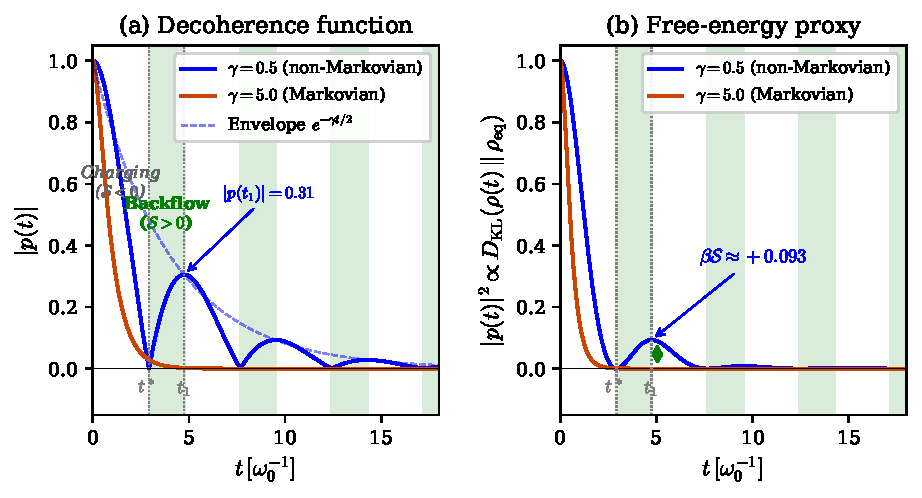
\includegraphics[width=\textwidth]{fig_survival.pdf}
\caption{%
Pure-dephasing spin-boson model
(Section~\ref{sec:example}) with Lorentz--Drude spectral
density~\eqref{eq:lorentz_drude}.
\textbf{Parameters:}
$\omega_0 = 1$ (energy unit),
$\lambda = 1$ (reorganization energy).
\textbf{Units:}
all times in $\omega_0^{-1}$;
energies in $\hbar\omega_0$.
\textbf{Regime:}
low temperature ($\beta\omega_0 \gg 1$);
the standard $T \to 0$ analytic
expression~\eqref{eq:decoherence}~\cite{BreuerPetruccione2002}
is used as an accurate proxy.
\textbf{(a)}~Decoherence amplitude $|p(t)|$
(eq.~\eqref{eq:decoherence}).
Blue: non-Markovian
($\gamma = 0.5$, $\gamma/4\lambda = 0.125$).
Orange: Markovian
($\gamma = 5.0$, $\gamma/4\lambda = 1.25$).
Dashed: exponential envelope $e^{-\gamma t/2}$.
Green bands indicate backflow
(Remark~\ref{rem:NM_regime}:
$d|p|/dt > 0$, $\Gamma(t) < 0$
per~\eqref{eq:Gamma_inst}).
\textbf{(b)}~Survival proxy
$|p(t)|^2 \propto \beta\,\mathcal{S}$
(eq.~\eqref{eq:S_qubit}).
At the first revival
($t_1 = \pi/\Omega \approx 4.75\,\omega_0^{-1}$),
the non-Markovian agent achieves
$\beta\,\mathcal{S}[t^*,t_1] \approx +0.093$
(eq.~\eqref{eq:S_numeric}), consistent with the
closed-form prediction~\eqref{eq:revival_exact},
funded by the consumption of pre-existing
correlations
(Proposition~\ref{prop:full_cycle}).
The Markovian comparison decays monotonically:
$\mathcal{S} \leq 0$ in this autonomous model
(Theorem~\ref{thm:autonomous_ceiling}).%
}
\label{fig:survival}
\end{figure}

\textbf{Consistency with
Theorem~\ref{thm:advantage} and
Proposition~\ref{prop:full_cycle}.}
Since this is autonomous evolution ($H_{\mathrm{ctrl}} = 0$),
identity~\eqref{eq:advantage_auto} applies exactly:
$\beta\,\mathcal{S} = -\Delta I(S{:}E)
- \Delta D_{\mathrm{KL}}(\rho_E \| \rho_E^{\mathrm{th}})$.
The example realizes the \emph{correlation battery}
of Remark~\ref{rem:battery}, with the charge--discharge
decomposition of
Proposition~\ref{prop:full_cycle}:
\begin{itemize}
\item \textbf{Charging} ($[0, t^*]$, eq.~\eqref{eq:charge}):
  the system decoheres, building correlations
  $I(S{:}E;\, t^*) > 0$ at the cost of
  $\mathcal{S} < 0$.
\item \textbf{Discharging} ($[t^*, t_1]$,
  eq.~\eqref{eq:discharge}):
  the correlations are consumed
  ($\Delta I < 0$ over this interval),
  returning $\beta\,\mathcal{S} \approx +0.093 > 0$.
\end{itemize}
The bound~\eqref{eq:S_upper} is satisfied:
$\beta\,\mathcal{S}[t^*, t_1] = 0.093
\leq I(S{:}E;\, t^*)$.
Full-cycle closure~\eqref{eq:full_cycle} is confirmed:
$\beta\,\mathcal{S}[0, t_1] < 0$.

\textbf{Instantaneous decoherence rate.}
The rate of coherence loss is
\begin{equation}
\label{eq:Gamma_inst}
\Gamma(t) := -\frac{d}{dt}\ln|p(t)|
= \frac{\gamma}{2}
  - \frac{\Omega\sin(\Omega t)
    + \tfrac{\gamma}{2}\cos(\Omega t)}
  {\cos(\Omega t)
    + \tfrac{\gamma}{2\Omega}\sin(\Omega t)}\,.
\end{equation}
In the Markovian limit $\gamma \gg 4\lambda$,
$\Gamma(t) \to \gamma/2 > 0$ for all $t$
(monotone decoherence).
In the non-Markovian regime $\gamma < 4\lambda$,
$\Gamma(t)$ oscillates and becomes \emph{negative}
during the backflow intervals where $|p(t)|$ increases.
These are precisely the intervals where
$\mathcal{S} > 0$.

\textbf{Closed-form revival amplitude.}
The decoherence function~\eqref{eq:decoherence} can be
written as $p(t) = R\, e^{-\gamma t/2}\cos(\Omega t - \phi)$,
where $R = \sqrt{1 + (\gamma/2\Omega)^2}$ and
$\phi = \arctan(\gamma/2\Omega)$, with $R\cos\phi = 1$.
The extrema of $|p(t)|$ occur at $t_n = n\pi/\Omega$
($n = 0, 1, 2, \ldots$), and the first revival peak
after the first zero is at $t_1 = \pi/\Omega$.
Its amplitude is \emph{exactly}
\begin{equation}
\label{eq:revival_exact}
|p(t_1)| = e^{-\gamma\pi/(2\Omega)},
\qquad
\beta\,\mathcal{S}[t^*, t_1]
\approx |p(t_1)|^2
= e^{-\gamma\pi/\Omega}.
\end{equation}
This is the paper's central computable prediction: the
survival gain at first backflow is determined by a single
dimensionless ratio $\gamma/\Omega$.

\begin{remark}[Parameter Survey]
\label{rem:parameter_survey}
Table~\ref{tab:survey} demonstrates the transition from
the Markovian regime ($\mathcal{S} \leq 0$) to the
non-Markovian regime ($\mathcal{S} > 0$) as the bath
memory rate $\gamma$ decreases below the critical value
$4\lambda$.
All entries use $\omega_0 = 1$, $\lambda = 1$,
$W = 0$ (autonomous evolution), with revival amplitudes
computed from~\eqref{eq:revival_exact}.
\begin{center}
\begin{tabular}{@{}cccccc@{}}
\toprule
$\gamma$ & $\gamma/4\lambda$ & Regime
& $|p(t_1)|$ & $\beta\,\mathcal{S}(t_1)$
& $\Gamma_{\min}$ \\
\midrule
$20.0$ & $5.0$ & Markov & --- & $\leq 0$ & $>0$ \\
$4.0$ & $1.0$ & Critical & --- & $\leq 0$ & $= 0$ \\
$2.0$ & $0.50$ & Non-Markov & $0.043$
  & $+0.002$ & $< 0$ \\
$1.0$ & $0.25$ & Non-Markov & $0.163$
  & $+0.027$ & $< 0$ \\
$0.5$ & $0.125$ & Deep NM & $0.305$
  & $+0.093$ & $< 0$ \\
$0.1$ & $0.025$ & Deep NM & $0.605$
  & $+0.37\phantom{0}$ & $< 0$ \\
\bottomrule
\end{tabular}
\end{center}
\captionsetup{hypcap=false}%
\captionof{table}{%
Survival functional at first backflow revival
as a function of the bath memory rate $\gamma$,
for the pure-dephasing spin-boson model
with Lorentz--Drude spectral density.
$|p(t_1)|$ is computed
from~\eqref{eq:revival_exact};
$\Gamma_{\min}$ is the sign of the minimum of the
instantaneous decoherence rate~\eqref{eq:Gamma_inst}.
The transition $\mathcal{S} \leq 0 \to \mathcal{S} > 0$
occurs precisely at the non-Markovian threshold
$\gamma = 4\lambda$.
For $\gamma = 0.1$ (deep non-Markovian),
the agent achieves $\beta\,\mathcal{S} \approx +0.37$
per backflow cycle in the autonomous setting
($H_{\mathrm{ctrl}} = 0$).%
}
\label{tab:survey}
\end{remark}

\begin{remark}[The Two Regimes: Summary]
\label{rem:two_regimes}
\begin{center}
\begin{tabular}{@{}lll@{}}
\toprule
& \textbf{Markovian ($\gamma = 20$)}
& \textbf{Non-Markovian ($\gamma = 0.5$)} \\
\midrule
$\gamma / 4\lambda$ & $5.0$ (overdamped)
  & $0.125$ (underdamped) \\
$\tau_B$ & $0.05\,\omega_0^{-1}$
  & $2.0\,\omega_0^{-1}$ \\
$p(t)$ & Monotone decay
  & Oscillatory with envelope \\
$|p(t_1)|$ at first revival & $0$ (no revival)
  & $\approx 0.31$ \\
$\beta\,\mathcal{S}$ at revival & $\leq 0$
  & $\approx +0.093$ \\
$\Gamma(t)$ & $> 0$ always
  & Oscillates, $< 0$ during backflow \\
Interpretation & Stone (sinks)
  & Surfer (rides backflow) \\
\bottomrule
\end{tabular}
\end{center}
The non-Markovian agent achieves
$\beta\,\mathcal{S} \approx +0.093$
per backflow cycle (autonomous, $H_{\mathrm{ctrl}} = 0$),
while the Markovian agent can only lose free energy.
As the coupling deepens ($\gamma/4\lambda \to 0$), the
revival amplitude grows and
$\mathcal{S}$ increases
(Table~\ref{tab:survey}), bounded above by
$\beta\,\mathcal{S} \leq I(S{:}E;\, t^*)$
(Corollary~\ref{cor:three_regimes}(iii)).
\end{remark}

% ============================================================
\section{The Cost of Memory}
\label{sec:cost}

The preceding identity allows a correlated initial resource to fund a
later interval.  It does not assign a universal energetic price to
storing or maintaining that resource.  This section separates
Landauer's erasure bound from a conditional archive-overload model used
only to motivate Paper~II.

\subsection{The Landauer Debt}

Landauer's principle prices a logically irreversible reset, not passive
storage, sensing, correlation maintenance, or reversible computation.

\begin{remark}[Conditional erasure cost]
\label{rem:landauer_scope}
If a declared memory implementation irreversibly erases
$N_{\mathrm{erase}}$ unbiased bits into a bath at temperature $T$, its
reset work obeys
\begin{equation}
\label{eq:landauer}
W_{\mathrm{reset}}\geq k_BT\ln2\,N_{\mathrm{erase}}.
\end{equation}
No lower bound proportional to total stored mutual information follows
without an implementation model.  Reversible storage and reversible
measurement can in principle avoid this reset cost until a logically
irreversible operation is performed~\cite{Landauer1961,Bennett1982}.
The former universal ``Landauer Cost of Memory'' proposition is
withdrawn.
\end{remark}

\subsection{Raw Archive Overload Scenario}

The crisis arises from the scaling of
$\mathcal{I}_{\mathrm{stored}}$ with time.
To quantify this, we borrow two quantities from computational
mechanics~\cite{CrutchfieldYoung1989,ShaliziCrutchfield2001}:

\begin{definition}[Entropy Rate and Predictive Information]
\label{def:entropy_rate}
Let $\{X_t\}$ be the stochastic process describing the
environment's influence on the agent (e.g., the sequence of
bath correlation values).
\begin{enumerate}
\item The \textbf{entropy rate} of the environment is
  \begin{equation}
  \label{eq:entropy_rate}
  h_\mu := \lim_{n \to \infty}
  H(X_n \mid X_{n-1}, \ldots, X_1),
  \end{equation}
  measuring the intrinsic unpredictability per time step.
\item The \textbf{predictive information} (excess entropy) is
  \begin{equation}
  \label{eq:pred_info}
  I_{\mathrm{pred}} := I(\overleftarrow{X};\,
  \overrightarrow{X})
  = \sum_{k=1}^{\infty}
  \bigl[H(X_k) - h_\mu\bigr],
  \end{equation}
  where $\overleftarrow{X}$ and $\overrightarrow{X}$ denote
  the past and future half-chains.
  This is the total amount of information about the future
  that is encoded in the past---the \emph{useful} memory.
\end{enumerate}
\end{definition}

Finite predictive information does not by itself prove that a finite
physical memory captures every useful feature, and positive entropy
rate does not lower-bound predictive information by
$h_\mu\tau_{\mathrm{mem}}$.  In particular, a stationary mixing
process commonly has finite excess entropy.

\begin{remark}[Conditional archive-overload scenario]
\label{rem:archive_overload}
Consider a deliberately specified implementation: an uncompressed raw
archive receives records at rate $r_{\mathrm{raw}}$ bits per unit time,
has capacity $M$ bits, and evaluates the entire archive once per control
cycle.  Without deletion it fills after $M/r_{\mathrm{raw}}$.  If it
irreversibly resets discarded records at rate $r_{\mathrm{erase}}$,
Landauer gives
\begin{equation}
\label{eq:mem_cost_rate}
\dot W_{\mathrm{reset}}\geq
k_BT\ln2\,r_{\mathrm{erase}}.
\end{equation}
For a long-memory or non-stationary source with divergent
$I_{\mathrm{pred}}$, the amount of predictively relevant history may
also grow, but that is an additional source assumption.  This archive
can exceed a finite storage, throughput, or reset budget.  The result is
an engineering overload scenario, not a universal thermodynamic
catastrophe and not a theorem that every memory implementation must
compress.
\end{remark}

\subsection{Conditional Motivation for Compression}

An agent using the raw-archive implementation may respond by increasing
capacity, lowering sample rate, reversible uncomputation, sufficient
statistics, lossy compression, or accepting stale data.  Paper~II
studies one coordinate-selection model among these options.

\begin{itemize}
\item \textbf{Compression requires a criterion.}
  To decide what to keep and what to erase, the agent needs a
  \emph{relevance function}---a mapping from stored correlations
  to survival value.
  This is a reference frame that ranks information by its
  contribution to $\mathcal{S}$.

\item \textbf{Coordinate selection uses a reference frame.}
  If the admissible compressor is restricted to retaining a subset of
  supplied coordinates, choosing that subset privileges a basis.  More
  general invariant or learned sufficient-statistic compressors need
  not have this form.
\end{itemize}

\begin{remark}[The Origin of Paper II]
\label{rem:paper_II}
Remark~\ref{rem:archive_overload} supplies Paper~II with a conditional
motivation: a bounded agent attempting to evaluate an uncompressed
archive needs some resource-allocation policy.  It does not prove that
compression, Clifford coordinates, spontaneous symmetry breaking, or a
``self'' is thermodynamically necessary.  Those are modelling choices
to be assessed in Paper~II.
\end{remark}

% ============================================================
\section{Numerical Demonstration}
\label{sec:numerical}

The preceding sections establish an autonomous thermodynamic baseline
and an accounting identity.  The following HMM is a separate classical
performance illustration: it compares finite observation windows with
a Bayes filter in an aliased environment.  Reward here is not the
thermodynamic survival functional, so the demonstration does not test
either theorem.
Full code and parameters are provided for reproducibility.

% ------------------------------------------------------------
\subsection{Model}
\label{subsec:demo_model}

\paragraph{Environment.}
A two-hidden-state HMM with aliased observations.
The hidden state $s_t \in \{0,1\}$ evolves as a persistent
Markov chain with $\Pr(s_{t+1} = s_t) = 1 - \varepsilon$;
the parameter $\varepsilon \in [10^{-3}, 10^{-1}]$ controls
the correlation length $\ell \sim 1/\varepsilon$.
Observations $o_t \in \{A, B\}$ are aliased:
$\Pr(o_t = A \mid s_t = 0) = 0.5 + \delta$,
$\Pr(o_t = A \mid s_t = 1) = 0.5 - \delta$,
with $\delta = 0.05$ (mutual information
$I(O; S) \approx 0.007$~bits).
Reward: $r_t = 1$ if $a_t = s_t$, $0$ otherwise.

\paragraph{Agents.}
All agents use the true model parameters and compute
exact Bayesian posteriors; the only difference is how many
observations each agent retains.
\begin{itemize}
\item \textbf{Markov-$k$} ($k \in \{1,2,4,8\}$): runs
  an exact Bayes filter over the most recent $k$
  observations (sliding window, uniform prior at each
  window start); acts by MAP.
\item \textbf{Memory (Bayes filter)}: maintains the full
  belief state $b_t = \Pr(s_t = 1 \mid o_{1:t})$ via the
  exact predict--update cycle over all past observations;
  acts by MAP.
\end{itemize}

\paragraph{Parameters.}
\begin{center}
\small
\begin{tabular}{@{}lcl@{}}
\toprule
\textbf{Quantity} & \textbf{Value} & \textbf{Role} \\
\midrule
$T$ & $100{,}000$ & horizon per trial \\
Seeds & 10 & independent replications \\
$\delta$ & 0.05 & observation asymmetry \\
$k$ & $\{1, 2, 4, 8\}$ & Markov window sizes \\
$\varepsilon$ & logspace($10^{-3}$, $10^{-1}$, 15)
  & transition noise grid \\
Burn-in & $5{,}000$ & discarded steps \\
\bottomrule
\end{tabular}
\end{center}

% ------------------------------------------------------------
\subsection{Results}
\label{subsec:demo_results}

Figure~\ref{fig:markov_ceiling} shows the two key signatures.

\paragraph{Result 1: finite-window performance saturation
(Figure~\ref{fig:markov_ceiling}a).}
The average reward $\bar{R}$ of the Bayes filter (memory
agent) increases monotonically with correlation length
$\ell = 1/\varepsilon$, while each Markov-$k$ agent
saturates at a distinct ceiling.  The ceilings are
ordered: $k = 1$ (lowest) through $k = 8$ (highest),
and all fall below the memory agent for
$\ell \gtrsim 20$.  This is a property of the specified
aliased HMM and agent classes, not a consequence of the
thermodynamic ceiling.

\paragraph{Result 2: Memory advantage
(Figure~\ref{fig:markov_ceiling}b).}
The gap $\Delta\bar{R} = \bar{R}_{\mathrm{mem}}
- \bar{R}_{\mathrm{Markov}\text{-}k}$ increases
monotonically with $\ell$, and is larger for smaller $k$.
Shaded bands show 95\% confidence intervals across
10 seeds.  The Markov-1 and Markov-2 curves nearly
overlap at small $\ell$, reflecting the fact that
short observation windows provide negligible additional
information in this aliasing regime---a consistency
check, not a deficiency.

\begin{figure}[t]
\centering
\includegraphics[width=\textwidth]%
  {fig_paper1_markov_ceiling.pdf}
\caption{%
\textbf{Finite-window saturation and Bayes-filter advantage.}
$T = 100{,}000$, 10 seeds, 95\% CI bands.
\textbf{(a)}~Average reward $\bar{R}$ vs correlation
length $\ell = 1/\varepsilon$.  The Bayes filter
(blue, bold) rises monotonically; Markov-$k$ agents
saturate at $k$-dependent ceilings.
\textbf{(b)}~Performance gap
$\Delta\bar{R} = \bar{R}_{\mathrm{mem}}
- \bar{R}_{\mathrm{Markov}\text{-}k}$
increases with $\ell$; smaller $k$ yields a larger gap.}
\label{fig:markov_ceiling}
\end{figure}

% ------------------------------------------------------------
\subsection{Scope of This Demonstration}
\label{subsec:demo_scope}

These simulations illustrate finite-window saturation under the stated
model class; they do not constitute a thermodynamic test.

\medskip
This demonstration \textbf{does} show:
\begin{enumerate}
\item A reproducible regime in which finite-order Markov
  agents exhibit a performance ceiling while a
  memory-carrying (Bayes filter) agent improves.
\item The performance gap widens with correlation length and tightens
  with window size in this HMM.  This is conceptually related to
  retained history but is not the quantity in
  Theorem~\ref{thm:advantage}.
\end{enumerate}

\noindent
This demonstration does \textbf{not} show:
\begin{enumerate}
\item Universality across environments, observation models,
  or agent architectures.  The model uses a two-state
  HMM with binary aliased observations.
\item Tight constants or the functional form of the
  ceiling boundary $\ell_c(k)$.
\item That the Bayes filter is optimal among all possible
  memory-carrying agents.
\end{enumerate}

\paragraph{Reproducibility.}
\begin{sloppypar}
The complete simulation is a self-contained Python script
(\texttt{paper1\_markov\_ceiling\_demo.py}, ${\sim}\,560$
lines, requiring only NumPy and Matplotlib) with fixed
random seeds.  All figures in this section can be
reproduced by executing the script.  The following files
are included in the supplementary archive:
\begin{itemize}
\item \texttt{paper1\_markov\_ceiling\_demo.py} --- simulation script
\item \texttt{fig\_paper1\_markov\_ceiling.pdf} --- Figure~\ref{fig:markov_ceiling}
\item \texttt{markov\_ceiling\_data.csv} --- raw sweep data
\item \texttt{markov\_ceiling\_boundary.csv} --- extracted
  ceiling boundaries $\ell_c(k)$
\end{itemize}
\end{sloppypar}

% ============================================================
\section{Discussion}
\label{sec:discussion}

\subsection{Summary of Results}

\begin{center}
\small
\setlength{\tabcolsep}{4pt}%
\begin{tabular}{@{}lP{7.5cm}c@{}}
\toprule
\textbf{Result} & \textbf{Statement} & \textbf{Sec.} \\
\midrule
Restricted autonomous ceiling &
  $\mathcal{S} \leq 0$ for a fixed-Hamiltonian Davies semigroup
  & \ref{sec:ceiling} \\[3pt]
Initial-resource balance &
  $\beta\mathcal{S} = -\Delta I
  - \Delta D_{\mathrm{KL}}
  - \beta\Delta\langle H_{\mathrm{ctrl}}\rangle
  - \beta\Delta\langle H_{\mathrm{int}}\rangle$
  & \ref{sec:advantage} \\[3pt]
Quantitative demo &
  Spin-boson: $\beta\mathcal{S} \approx +0.093 > 0$
  at first backflow revival (Fig.~\ref{fig:survival},
  Table~\ref{tab:survey})
  & \ref{sec:example} \\[3pt]
Memory/record interface &
  operational influence relation plus a conditional record test
  & \ref{sec:arrow} \\[3pt]
Archive overload &
  conditional on raw storage, finite capacity, and irreversible reset
  & \ref{sec:cost} \\[3pt]
Numerical demo &
  finite-window saturation in an aliased HMM
  (Fig.~\ref{fig:markov_ceiling})
  & \ref{sec:numerical} \\
\bottomrule
\end{tabular}
\end{center}

\subsection{What This Paper Does and Does Not Show}

\textbf{This paper shows:}
\begin{enumerate}
\item Under an autonomous fixed-Hamiltonian Davies semigroup,
  the survival functional $\mathcal{S} \leq 0$
  (Theorem~\ref{thm:autonomous_ceiling}).
\item For any initial state (product or correlated), the
  survival functional satisfies the exact identity
  $\beta\,\mathcal{S} = -\Delta I(S{:}E)
  - \Delta D_{\mathrm{KL}}(\rho_E \| \rho_E^{\mathrm{th}})
  - \beta\,\Delta\langle H_{\mathrm{ctrl}}\rangle
  - \beta\,\Delta\langle H_{\mathrm{int}}\rangle$
  (Theorem~\ref{thm:advantage}).
  Under autonomous evolution, when pre-existing
  system--environment correlations are consumed
  ($\Delta I < 0$), $\mathcal{S} > 0$ is achievable,
  bounded by the initial correlation budget
  (Corollary~\ref{cor:three_regimes}).
\item A quantitative spin-boson example illustrates:
  $\beta\,\mathcal{S} \approx +0.093 > 0$ at the first
  non-Markovian revival (Section~\ref{sec:example}).
\item The memory-influence relation and HAFF record ordering define a
  conditional model test, not a proved embedding
  (Conjecture~\ref{prop:HAFF_bridge}).
\item Landauer supplies a conditional reset cost; a raw finite archive
  can overload under the implementation assumptions in
  Remark~\ref{rem:archive_overload}.
\item A computational demonstration exhibits finite-window saturation
  in a two-state HMM with aliased observations
  (Section~\ref{sec:numerical},
  Figure~\ref{fig:markov_ceiling}).
\end{enumerate}

\textbf{This paper does not show:}
\begin{enumerate}
\item That memory or non-Markovianity is necessary or sufficient for
  persistence.
\item That non-Markovian systems optimize a larger survival supremum
  than all Markovian systems.
\item That driven or measurement-feedback Markovian agents obey the
  restricted autonomous ceiling (Remark~\ref{rem:driven_protocol}).
\item That the specific form of the optimal memory kernel can be
  derived from first principles without specifying the
  environment.
\item That memory implies or requires consciousness.
\item That storage or maintenance has a universal Landauer cost, or
  that compression and symmetry breaking are thermodynamic necessities.
\end{enumerate}

% ============================================================
% REFERENCES
% ============================================================
\begin{thebibliography}{99}

\bibitem{BreuerPetruccione2002}
H.-P.~Breuer and F.~Petruccione,
\emph{The Theory of Open Quantum Systems},
Oxford University Press (2002).

\bibitem{Schrodinger1944}
E.~Schr\"odinger,
\emph{What is Life?},
Cambridge University Press (1944).

\bibitem{Lindblad1976}
G.~Lindblad,
\emph{On the generators of quantum dynamical semigroups},
Commun.\ Math.\ Phys.\ \textbf{48}, 119 (1976).

\bibitem{GKS1976}
V.~Gorini, A.~Kossakowski, and E.~C.~G.~Sudarshan,
\emph{Completely positive dynamical semigroups of $N$-level systems},
J.\ Math.\ Phys.\ \textbf{17}, 821 (1976).

\bibitem{Nakajima1958}
S.~Nakajima,
\emph{On quantum theory of transport phenomena},
Prog.\ Theor.\ Phys.\ \textbf{20}, 948 (1958).

\bibitem{Zwanzig1960}
R.~Zwanzig,
\emph{Ensemble method in the theory of irreversibility},
J.\ Chem.\ Phys.\ \textbf{33}, 1338 (1960).

\bibitem{SagawaUeda2010}
T.~Sagawa and M.~Ueda,
\emph{Generalized Jarzynski Equality under Nonequilibrium Feedback Control},
Phys.\ Rev.\ Lett.\ \textbf{104}, 090602 (2010).

\bibitem{SagawaUeda2012}
T.~Sagawa and M.~Ueda,
\emph{Fluctuation Theorem with Information Exchange},
Phys.\ Rev.\ Lett.\ \textbf{109}, 180602 (2012).

\bibitem{RivasHuelgaPlenio2014}
\'{A}.~Rivas, S.~F.~Huelga, and M.~B.~Plenio,
\emph{Quantum non-Markovianity: characterization, quantification and detection},
Rep.\ Prog.\ Phys.\ \textbf{77}, 094001 (2014).

\bibitem{Spohn1978}
H.~Spohn,
\emph{Entropy production for quantum dynamical semigroups},
J.\ Math.\ Phys.\ \textbf{19}, 1227 (1978).

\bibitem{Landauer1961}
R.~Landauer,
\emph{Irreversibility and heat generation in the computing process},
IBM J.\ Res.\ Dev.\ \textbf{5}, 183 (1961).

\bibitem{Bennett1982}
C.~H.~Bennett,
\emph{The thermodynamics of computation---a review},
Int.\ J.\ Theor.\ Phys.\ \textbf{21}, 905 (1982).

\bibitem{BreuerLainePiilo2009}
H.-P.~Breuer, E.-M.~Laine, and J.~Piilo,
\emph{Measure for the Degree of Non-Markovian Behavior of Quantum Processes in Open Systems},
Phys.\ Rev.\ Lett.\ \textbf{103}, 210401 (2009).

\bibitem{EspositoLindenbergVandenBroeck2010}
M.~Esposito, K.~Lindenberg, and C.~Van~den~Broeck,
\emph{Entropy production as correlation between system and reservoir},
New J.\ Phys.\ \textbf{12}, 013013 (2010).

\bibitem{Zurek2009}
W.~H.~Zurek,
\emph{Quantum Darwinism},
Nature Physics \textbf{5}, 181 (2009).

\bibitem{CrutchfieldYoung1989}
J.~P.~Crutchfield and K.~Young,
\emph{Inferring statistical complexity},
Phys.\ Rev.\ Lett.\ \textbf{63}, 105 (1989).

\bibitem{ShaliziCrutchfield2001}
C.~R.~Shalizi and J.~P.~Crutchfield,
\emph{Computational mechanics: Pattern and prediction, structure and simplicity},
J.\ Stat.\ Phys.\ \textbf{104}, 817 (2001).

\bibitem{BialekNemenmanTishby2001}
W.~Bialek, I.~Nemenman, and N.~Tishby,
\emph{Predictability, complexity, and learning},
Neural Computation \textbf{13}, 2409 (2001).

\bibitem{Liu2026HAFF_A}
S.~Liu, \emph{Emergent Geometry from Coarse-Grained Observable Algebras: The Holographic Alaya-Field Framework}, Zenodo (2026), DOI: 10.5281/zenodo.18361706.

\bibitem{Liu2026HAFF_B}
S.~Liu, \emph{Accessibility, Stability, and Emergent Geometry: Conceptual Clarifications on the Holographic Alaya-Field Framework}, Zenodo (2026), DOI: 10.5281/zenodo.18367060.

\bibitem{Liu2026HAFF_C}
S.~Liu, \emph{Causation, Agency, and Existence: Structural Constraints and Interpretive Bridges}, Zenodo (2026), DOI: 10.5281/zenodo.18374805.

\bibitem{Liu2026HAFF_F}
S.~Liu, \emph{Accessibility Propagation and Temporal Direction: A Conditional Structural Analysis}, Zenodo (2026), DOI: 10.5281/zenodo.18400425.

\bibitem{Liu2026QRAIF_A}
S.~Liu, \emph{A Clifford-Encoding Model for Lorentzian Metrics in Entropic Gravity Frameworks}, Zenodo (2026), DOI: 10.5281/zenodo.18525876.

\bibitem{Liu2026QRAIF_B}
S.~Liu, \emph{Thermodynamic Stability Constraints on the Operator Algebra of Persistent Open Quantum Subsystems}, Zenodo (2026), DOI: 10.5281/zenodo.18525890.

\end{thebibliography}

\end{document}
